%!TEX program=xelatex
\documentclass[a4paper]{ctexrep}
 %%%%%%%%%%%%  Include Packages  %%%%%%%%%%%%%%
\usepackage{fancyhdr}
\usepackage[colorlinks, linkcolor=black]{hyperref}
\usepackage{listings, geometry, amsmath, graphicx, tabularx, topcapt}
\usepackage[colorinlistoftodos]{todonotes}
\usepackage{adjustbox}
\usepackage{tikz}
\usetikzlibrary{circuits.logic.US}
\tikzstyle{branch}=[fill,shape=circle,minimum size=2pt,inner sep=0pt]
\def\srdefaultlength{0.5cm}
\usepackage{booktabs}
\usepackage{longtable}
\usepackage{lipsum}
\usepackage{float}
\usepackage{multirow}
\usepackage{fancyvrb}
\usepackage[section]{placeins}% force float within subsection
%%%%%%%%%%%%%%%  Color and Fonts  %%%%%%%%%%%%%%%%%%

\definecolor{mygreen}{rgb}{0,0.6,0}
\definecolor{mygray}{rgb}{0.5,0.5,0.5}
\definecolor{mymauve}{rgb}{0.58,0,0.82}

\definecolor{dkgreen}{rgb}{0,0.6,0}
\definecolor{gray}{rgb}{0.5,0.5,0.5}
\definecolor{mauve}{rgb}{0.58,0,0.82}

\lstset{frame=tb,
  language=Python,
  aboveskip=3mm,
  belowskip=3mm,
  showstringspaces=false,
  columns=flexible,
  basicstyle={\small\ttfamily},
  numbers=none,
  numberstyle=\tiny\color{gray},
  keywordstyle=\color{blue},
  commentstyle=\color{dkgreen},
  stringstyle=\color{mauve},
  breaklines=true,
  breakatwhitespace=true,
  tabsize=3
}

\geometry{left=3cm,right=3cm,top=4cm,bottom=5cm}

\hypersetup{
	pdftitle={人工智能实验报告},
	pdfauthor={胡博涵},
	pdfsubject={人工智能},
	pdfkeywords={},
}

\ctexset {
	section = {
		number = \arabic{section},
		format = \Large\bfseries,
	},
	subsection = {
		number = \arabic{section}.\arabic{subsection},
	}
}

%%%%页眉页脚
\title{人工智能实验报告}
\begin{document}
	\begin{titlepage} % 封面
		\begin{center}
                        
\includegraphics[width=5cm]{xh.png}\\[0.5cm]
        		
\includegraphics[width=7cm]{logo.png}\\[0.5cm]
                		{\zihao{0} \heiti \textbf{\uline{人~工~智~能~实~验~报~告}}\\[0.5cm]}		
        		 %{\zihao{1} \fangsong \textbf{搜索策略}}		
        		\vfill
        		\vfill
        		\vfill
        		\vfill
        		\vfill
        		\vfill
        		\vfill
        		\vfill
        		\vfill
        		\vfill
        		\vfill
        		\vfill		
                \vfill        		
                \vfill
        		{\zihao{3}\songti
        		\begin{tabular}{lc}
                    开课学期& {\uline{\hfill 大三上学期\hfill}}\\
                    课程名称& {\uline{\hfill 人工智能\hfill}}\\
                    实验名称& {\uline{\hfill 知识表示\hfill}}\\
                    实验性质& {\uline{\hfill 设计\hfill}}\\
                    实验时间& {\uline{\hfill 2019.10\hfill}}\\
                    地~~~~~~点& {\uline{\hfill \textbf{T2}102\hfill}}\\
                    学生专业& {\uline{\hfill 计算机\hfill}}\\
                    学生学号& {\uline{\hfill SZ170110113\hfill}}\\
                    学生姓名& {\uline{\hfill 胡博涵\hfill}}\\
                    批阅教师& {\uline{\hfill \hfill}}\\
                    报告成绩& {\uline{\hfill \hfill}}\\

        		\end{tabular}		}
        		\vfill	
		实验与创新实践教育中心印制\\
2019年10月

		\end{center}
	\end{titlepage}


%%%%%%%%%%%%%%%%%%%  目录  %%%%%%%%%%%%%%%%%%%%%	
	
%\setcounter{tocdepth}	% 目录深度到 \section{} 为止
\tableofcontents % 内容目录
\pagebreak

%\listoffigures % 图片目录
%\pagebreak

%\listoftables  %表格目录
%\pagebreak

%%%%%%%%%%%%%% 正文  %%%%%%%%%%%%%%%%%

%
\pagestyle{fancy}
\lhead{}% 使用lhead 定义左侧上方页眉
\chead{人工智能实验报告}% 使用rhead 定义右侧上方页眉
\rhead{}
\lfoot{}% 使用lfoot 定义左侧下方页脚
\cfoot{\thepage}% 使用cfoot 定义下方中间页脚
\rfoot{}% 使用rfoot 定义右侧下方页脚
\renewcommand{\headrulewidth}{0.2pt}
\renewcommand{\footrulewidth}{0.4pt}

\section{简介/问题描述}
\subsection{待解决问题的解释}
\par 一个房间里,天花板上挂有一串香蕉,房间里有一个箱子,有一只猴子可以到处走动、推移箱子、攀登箱子。当箱子在香蕉下方,猴子在箱子上时,猴子才可以摘到香蕉。求解猴子在某一状态下(设猴子位置为A,箱子位置为B,香蕉位置在C,摘取到香蕉的步骤序列。

\subsection{问题的形式化描述}
\par 设猴子的位置为M,香蕉位置为B,箱子位置为Box,On表示猴子是否在箱子上,H表示猴子是否摘到香蕉,则问题可形式化为:对于给定的$(M_0, B_0, Box_0, On_0, H_0)$,制定一系列状态转移的规则,使状态通过这一系列的规则进行转移,状态达到$(M_n, B_n, Box_n, On_n, H = 1)$的状态,并记录下这一操作序列。
\subsection{解决方案介绍(原理)}
\par 采用产生式方法解决这个问题。产生式系统的基本结构包括三个组成部分:综合数据库、规则库和控制系统。
\par 其中,综合数据库存储推理过程中的当前信息,作为推理过程中选择可用规则的依据,以决定下一步的操作。存储的信息可以是问题的初始状态(猴子、箱子和香蕉的初始位置)、可以是通过推理规则得到的问题的中间状态(猴子、箱子和香蕉在某一时刻的位置)。
\par 规则库存储推理所需的所有规则,控制系统则选择适用的推理规则进行推理,并记录当前的规则序列。


\section{算法介绍}
\subsection{所用方法的一般介绍}
\paragraph{产生式系统} 产生式系统的知识表示方法分为状态的表示和推理规则的表示,其中,状态的表示可以使用一个五元组,$(Monkey, Box, Banana, Onbox, HB)$,其中,$Monkey, Box, Banana \in {A,B,C}$表示三者各自的位置。$OnBox,HB \in {0,1}$,表示猴子是否在箱子上、猴子是否拿到香蕉。
\par 对于本问题而言,由于解决的方法相对固定,即状态之间转移的形式比较统一,且问题的状态数较少,推理规则较为简单,故适合使用产生式系统来表示。
\par 对于本问题而言,推理规则和其优先级已经拥有了固定的形式,即:
\begin{enumerate}
  \item 如果猴子已经在箱子上,箱子在香蕉下,则摘香蕉
  \item 如果猴子和箱子的位置不同,则猴子需要先移动到箱子的位置
  \item 如果猴子、箱子、香蕉位置相同,猴子不在箱子上,则爬箱子
  \item 如果猴子、箱子位置相同,而和香蕉位置不同,则移动箱子到香蕉的位置
  \item 如果猴子已经在箱子上,然而箱子不在香蕉下面,则先爬下箱子
\end{enumerate}
\par 可以看到,我们充分考虑了各种边界情况,例如,初始状态,猴子在箱子上,而箱子却不在香蕉下面这种情况。
\paragraph{推理规则} 上述所列出的人工构造的推理规则形式规整,都是采用IF P THEN Q的形式,其中P和Q分别为状态集合中的状态,P为产生式的前提,给出产生式能否使用的先决条件,Q是一组结论或操作,表示P得到满足时,应该推出的结论和动作。整个产生式表示如果当前状态为P,则下一步应该转移到Q的状态。这种规则方便计算机表示。
产生式系统的一般运行规则如下:
\begin{lstlisting}
(1)	初始实时放入数据库
(2)	对数据库中的事实和事实进行匹配
(3)	若匹配成功:
        a)	将该事实放入数据库
        b)	执行规定的操作
(4)	若匹配不成功:
        a)	返回(2)
\end{lstlisting}


\subsection{算法伪代码}
\begin{lstlisting}
function solve(step):
    step += 1
    if state.HB == 1:
        return step
    if MonkeyPosition = BoxPosition = BananaPosition and OnBox:
        Monkey Grasp the Banana
        return solve(step)
    if MonkeyPosition != BoxPosition:
        Monkey Moves to the Box
        return solve(step)
    if MonkeyPosition = BoxPostion = BananaPosition and not OnBox:
        Monkey Climbs up the Box
        return solve(step)
    if MonkeyPosition = BoxPosition != BananaPosition and OnBox:
        Monkey Climbs down the Box
        return solve(step)
    if MonkeyPosition = BoxPosition != BananaPosition and not OnBox:
        Monkey Push the Box to the Position of Banana
        return solve(step)
\end{lstlisting}
\section{算法实现}

\subsection{实验环境与问题规模}
实验环境:Python 3.6 \\
问题规模:本问题规模较小,其中,状态的元组维数只有5个,推理用到的规则数量也只有5个。


\subsection{数据结构}
\paragraph{状态的表示} 状态使用五元组表示,$(Monkey, Box, Banana, Onbox, HB)$,在实现时,采用一个包含以上变量的类进行实现。
\paragraph{规则的表示} 规则的表示如下:
\begin{lstlisting}
r1: IF (x,y,a,0,0)  THEN  (y,y,a,0,0)	猴子移动
r2: IF (x,x,y,0,0)  THEN  (y,y,y,0,0)	猴子移动箱子
r3: IF (x,x,y,1,0)  THEN  (x,x,y,0,0)	猴子爬上箱子
r4: IF (x,x,x,0,0)  THEN  (x,x,x,1,0)	猴子爬下箱子
r5: IF (x,x,x,1,0)  THEN  (x,x,x,1,1)	猴子摘取香蕉
\end{lstlisting}
(有:$x,y,a \in {-1,0,1},x \neq y,a$任意)
\par 在具体实现时,采用一系列的if语句判断规则是否满足,若满足,则改变当前状态。
\subsection{实现方法}
\par 在产生式规则中,由于对于每一个状态,都有对应的转换规则。所以编写统一的函数action,通过一系列的IF语句,判断当前的状态,并选择相应的操作函数,改变当前的状态,并递归调用函数action函数,对下一个状态进行转移操作。
\begin{table}[H]
  \centering
  \caption{操作列表}
    \begin{tabular}{cc}
    \toprule
    操作函数  & 解释 \\
    \midrule
    monkeymove & 猴子移动到箱子的位置 \\
    monkeyclimb & 猴子爬上箱子 \\
    monkeydown & 猴子爬下箱子 \\
    monkeypush & 猴子推动箱子到香蕉的位置 \\
    grasp & 猴子摘取香蕉 \\
    \bottomrule
    \end{tabular}%
  \label{tab:addlabel}%
\end{table}%

\subsection{实验结果}
\par 测试了几种情况,运行结果均正确。
\begin{figure}[H]
  \centering
  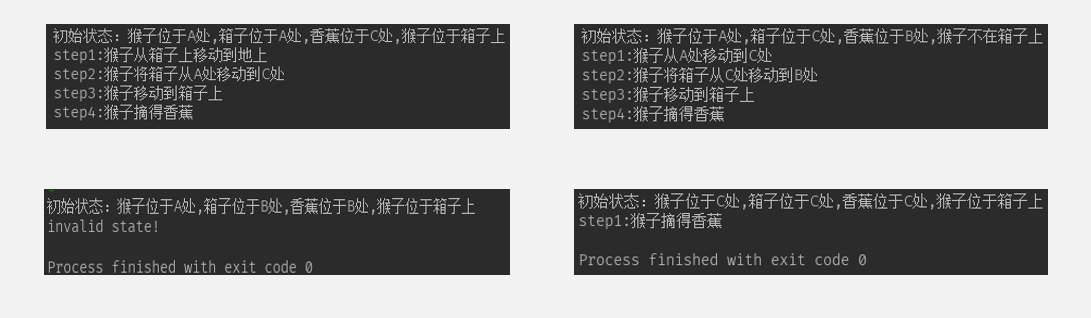
\includegraphics[scale=0.7]{1.png}
\end{figure}


\section{总结与讨论}
\par 本次实验,我们主要学习了知识表示方法的实现。知识的表示方法分为一阶谓词表示、产生式规则表示、语义网络表示和框架表示。
\par 通过讨论,我们发现猴子摘香蕉问题的结构特征明显,推理规则简单,状态空间小,非常适合使用产生式规则来表示。产生式系统的优点是状态定义方便,转移逻辑实现简单。
\par 产生式系统推理过程十分自然,采用“如果...,则...”的形式,和我们人类的判断基本一致。规则具有模块性,方便添加、删除和修改规则。
\par 但是产生式系统也有一定的缺点,产生式系统效率较低,每次选择规则时,都需要将规则和当前的状态进行一一匹配。

\section{附录:源代码及注释、小组分工及贡献度}
\begin{lstlisting}
小组成员都独自完成一版实验一。每个人的贡献度都是100%。
\end{lstlisting}
\begin{lstlisting}
state_flag = {-1: "A", 0: "B", 1: "C"}


class state:
    monkey = -2
    banana = -2
    box = -2
    onbox  = -2 #猴子在箱子上
    HB = -2     #猴子摘到香蕉


def init():
    state.monkey = int(input("MONKEY at A:-1/B:0/C:1\n"))
    state.banana = int(input("BANANA at A:-1/B:0/C:1\n"))
    state.box = int(input("BOX at A:-1/B:0/C:1\n"))
    state.onbox = int(input("on box? at Y:1/N:0\n"))
    state.HB = 0
    print("初始状态:猴子位于%c处,箱子位于%c处,香蕉位于%c处" % (state_flag[state.monkey], state_flag[state.box], state_flag[state.banana]),
          end=',')
    if state.onbox:
        print("猴子位于箱子上")
    else:
        print("猴子不在箱子上")

def init_ck():
    if (state.monkey != -1 and state.monkey != 0 and state.monkey != 1)  \
       or (state.banana != -1 and state.banana != 0 and state.banana != 1)  \
       or (state.box != -1 and state.box != 0 and state.box != 1)  \
       or (state.onbox != 0 and state.onbox != 1) \
       or (state.HB != 0 and state.HB != 1):
        print("invalid state!")
        exit(0)

    if state.monkey != state.box and state.onbox == 1:
        print("invalid state!")
        exit(0)
    if state.monkey != state.banana and state.HB == 1:
        print("invalid state!")
        exit(0)
    if state.monkey != state.banana and state.HB == 1:
        print("invalid state!")
        exit(0)



def monkeymove(step):
    print("step%d:猴子从%c处移动到%c处" % (step, state_flag[state.monkey], state_flag[state.box]))
    state.monkey = state.box


def monkeyclimb(step):
    state.onbox = 1
    print("step%d:猴子移动到箱子上" % (step,))


def monkeydown(step):
    state.onbox = 0
    print("step%d:猴子从箱子上移动到地上" % (step,))


def monkeypush(step):
    print("step%d:猴子将箱子从%c处移动到%c处" % (step, state_flag[state.box], state_flag[state.banana]))
    state.box = state.banana
    state.monkey = state.banana


def grasp(step):
    print("step%d:猴子摘得香蕉" % (step,))
    state.HB = 1


def action(step=0):
    step += 1
    if state.HB == 1:
        return step
    if state.monkey == state.box == state.banana and state.onbox == 1:
        grasp(step)
        return action(step)
    if state.monkey != state.box:
        monkeymove(step)
        return action(step)
    if state.monkey == state.box == state.banana and state.onbox == 0:
        monkeyclimb(step)
        return action(step)
    if state.monkey == state.box != state.banana and state.onbox == 1:
        monkeydown(step)
        return action(step)
    if state.monkey == state.box != state.banana and state.onbox == 0:
        monkeypush(step)
        return action(step)


if __name__ == "__main__":
    init()
    init_ck()
    action()
\end{lstlisting}





\end{document}
